\subsubsection{Higgs candidate pairing}
\label{subsubsec:higgs-pairing}

The \HH system is reconstructed from two \textit{Higgs candidates}, which are themselves reconstructed from two jets each (four \textit{Higgs candidate jets} in total). These jets are selected from the pool of central jets. \bjets are selected first. If the event is a 4b event, the leading four in \pt are selected. If it is a 2b event, the remaining places are filled by non-b-tagged jets, which are sorted in \pt and the two leading jets taken. For details on the \Pqb-tag based selection, see \Sect{\ref{sec:sel-btag}}.

We define \textbf{pairing} as the identification of a jet pair as a Higgs candidate. Given the four selected \textit{Higgs candidate jets}, three possible pairings are possible, as sketched in Figure \ref{fig:poss-pairs}. We must therefore devise a strategy that accurately predicts which pairing is correct. 
The \textbf{correct pairing} is defined with generator level information. First, \Pqb-quarks are matched to \Pqb-jets using a $\Delta R < 0.3$ criterion. The correct pair is then defined by the \Pqb-quarks which have the same parent barcode ID in the truth record.

The pairing method chosen in this iteration of the analysis is based on the principle that the decay products of the Higgs should show a degree of collimation due to the Higgs's initial momentum. Of the two Higgs boson candidates in a given pairing, the \textit{leading} Higgs candidate is defined as the one with the highest \pt. For each of the three pairing options, the leading Higgs candidate is identified and the $\Delta R_{Leading}(jj)$ between its two constituent jets calculated. 
The pairing option with the smallest $\Delta R_{Leading}(jj)$ is selected.
% The leading Higgs candidate associated with the smallest $\Delta R$ is selected. The remaining two jets are then taken as the other Higgs candidate.

\begin{figure}[b]
    \centering
    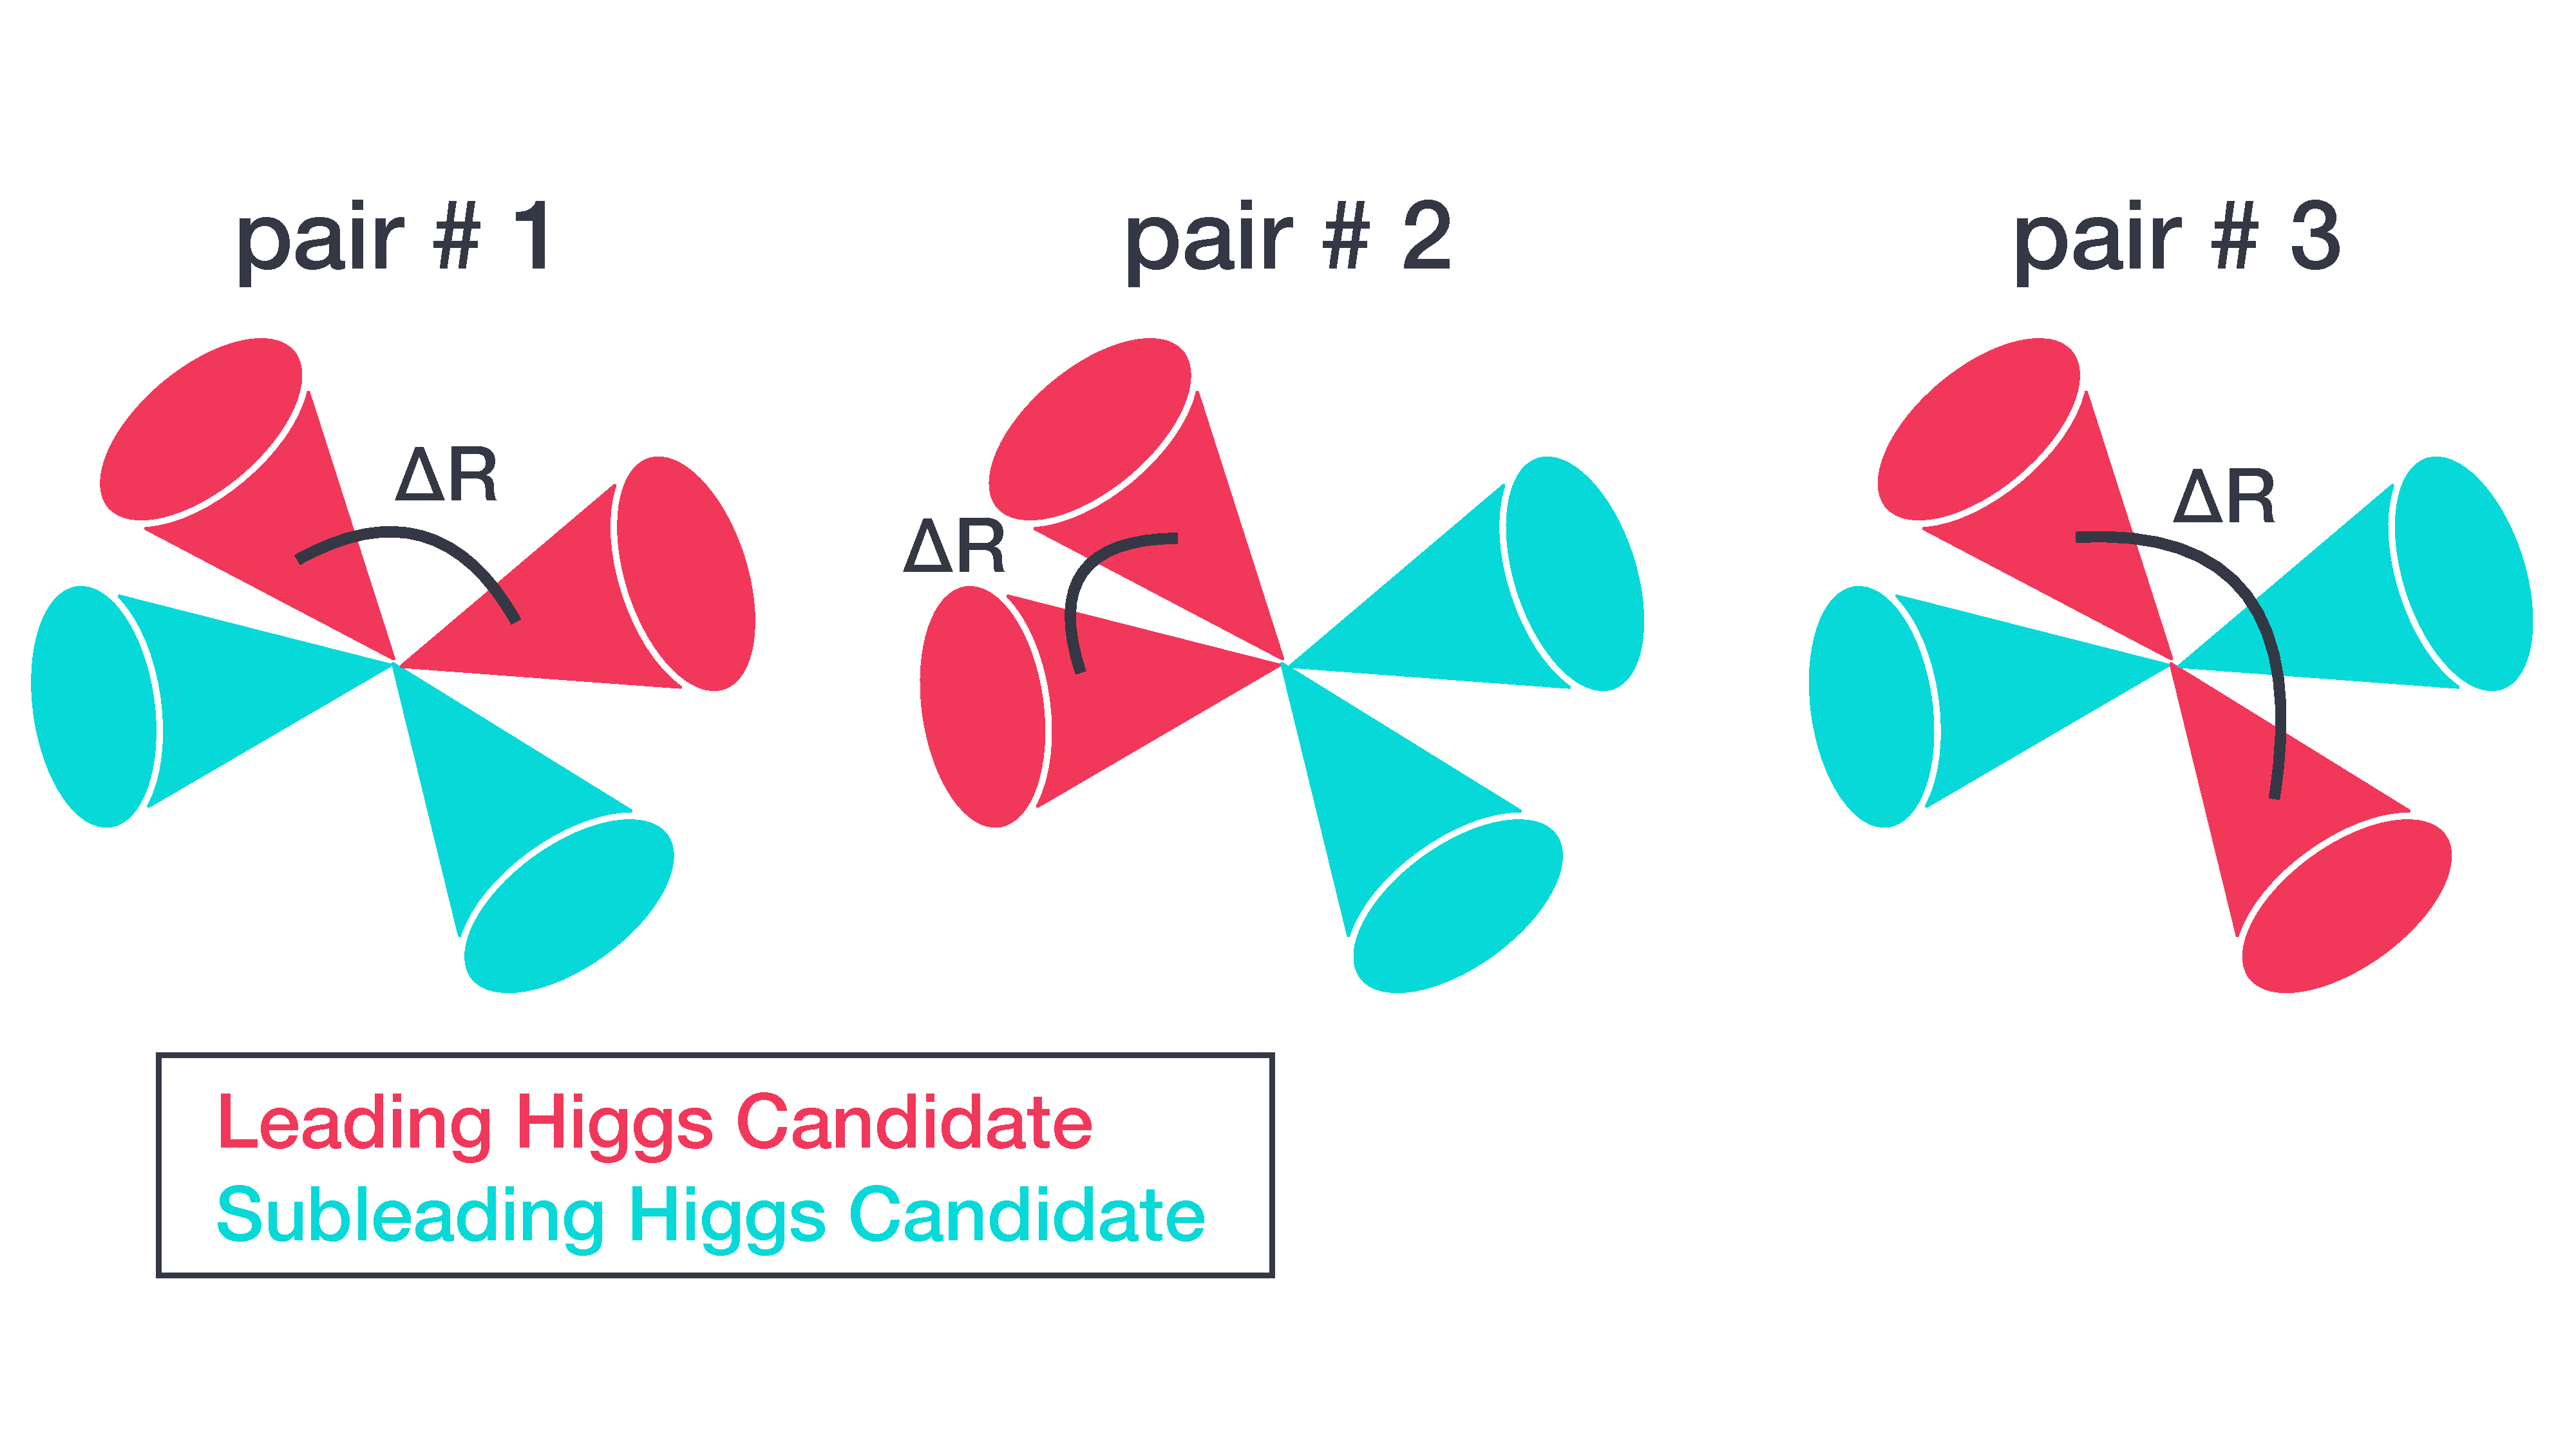
\includegraphics[width=0.8\textwidth,,trim=0 4cm 0 5cm,clip]{figures/nr-int-note/selection/V2/pairing.pdf}
    \caption{The three possible pairing permutations of the four \HH jets into the two Higgs candidates.  The opening angles between the jets in the leading Higgs Candidate are indicated, so pair number 2 is the selected pairing.}
    \label{fig:poss-pairs}
\end{figure}

\paragraph{Pairing accuracy} The pairing accuracy is defined as the fraction of correctly paired events among the events where the four Higgs-decayed jets are corrected selected by the jet selection. This definition is selected to decouple the pairing accuracy from the jet selection accuracy, as defined in \Sect{\ref{sec:sel-btag}}. The pairing accuracy is shown in \Fig{\ref{fig:pairingAcc-exists-4b}} as a function of \kl and \kvv, and in \Fig{\ref{fig:pairingAcc-mhh-exists-4b}} as a function of \mhh.
Signals with harder \pt Higgs tend to have more collimated jet pairs, resulting in higher pairing accuracies. 
This effect leads to a loss of accuracy for low $m_{HH}$ events (i.e., $m_{HH} < 450$ GeV), as also seen a drop of the pairing accuracy with non-SM \kl values or SM-like \kvv values as they lead to softer kinematics. This is deemed acceptable because most of the analysis background is also located at low $m_{HH}$, therefore losing these events do not reflect in a loss of performance.


\begin{figure}[hbt]
	\centering
	\subfloat[Pairing accuracy vs \kl]{
	     	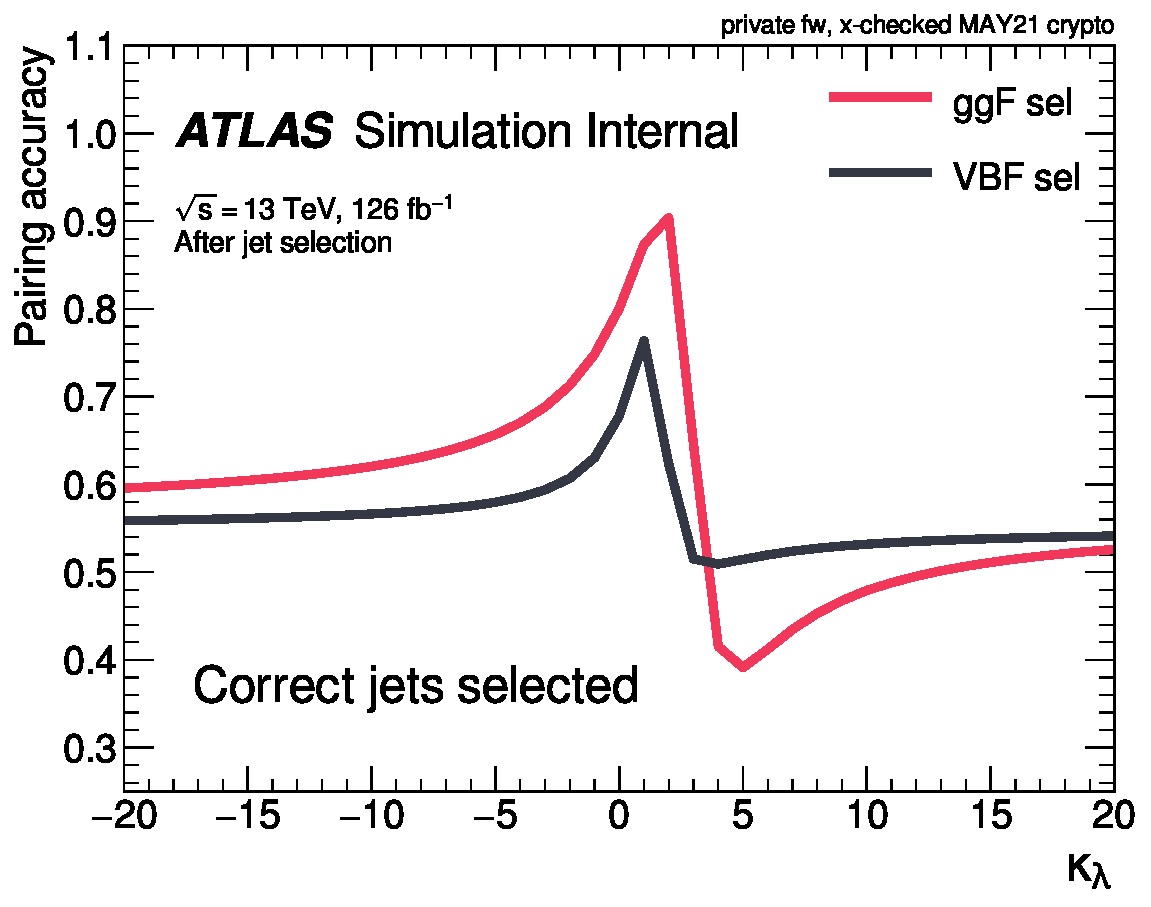
\includegraphics[width=0.4\textwidth]{figures/nr-int-note/selection/V2/acc_kl_exists_4b_only.pdf}
		\label{fig:pairingAcc-kl-exists-4b}
	}
	\subfloat[Pairing accuracy vs $\kappa_{2V}$]{
	     	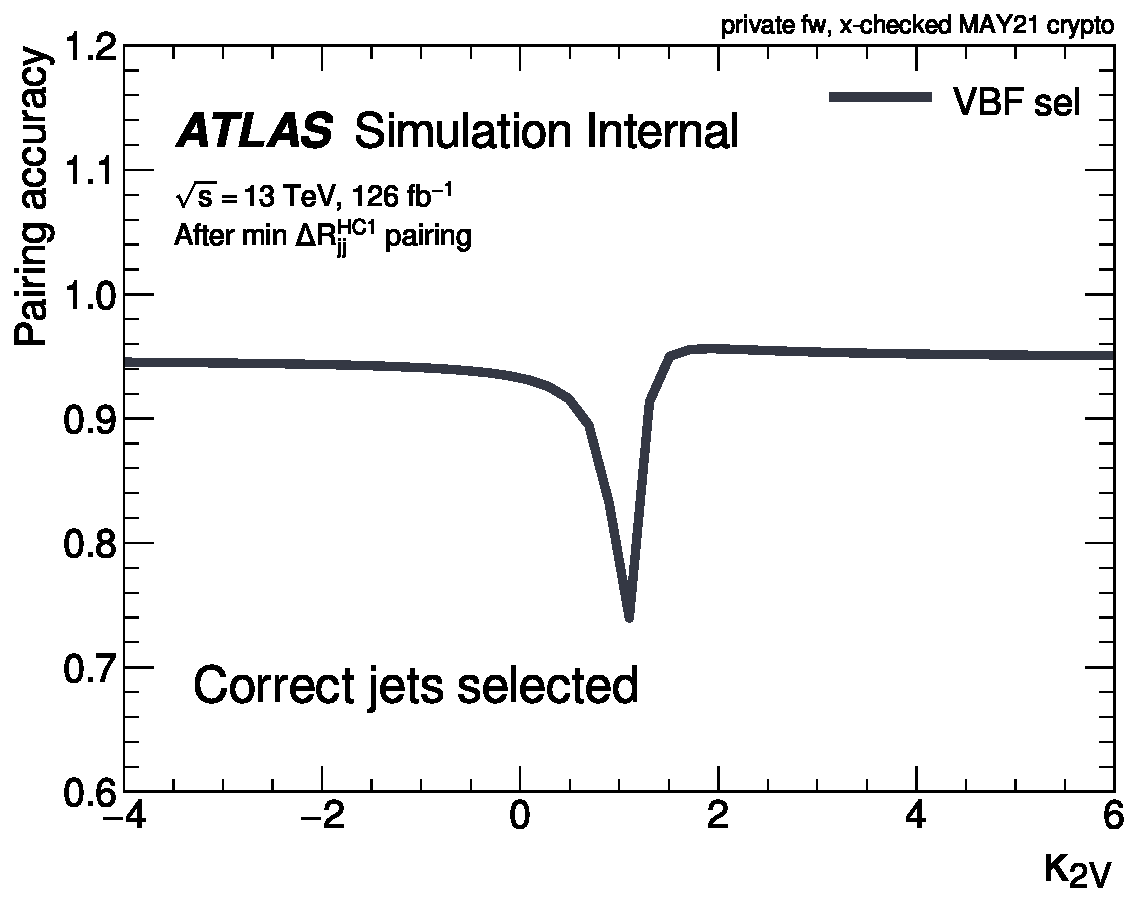
\includegraphics[width=0.4\textwidth]{figures/nr-int-note/selection/V2/acc_k2V_exists.pdf} 
		\label{fig:pairingAcc-k2V-exists}
	}
	\caption{The pairing accuracy as a function of \kl and \kvv, given that the correct jets have been selected.}
	\label{fig:pairingAcc-exists-4b}
\end{figure}

\begin{figure}[b]
    \centering
    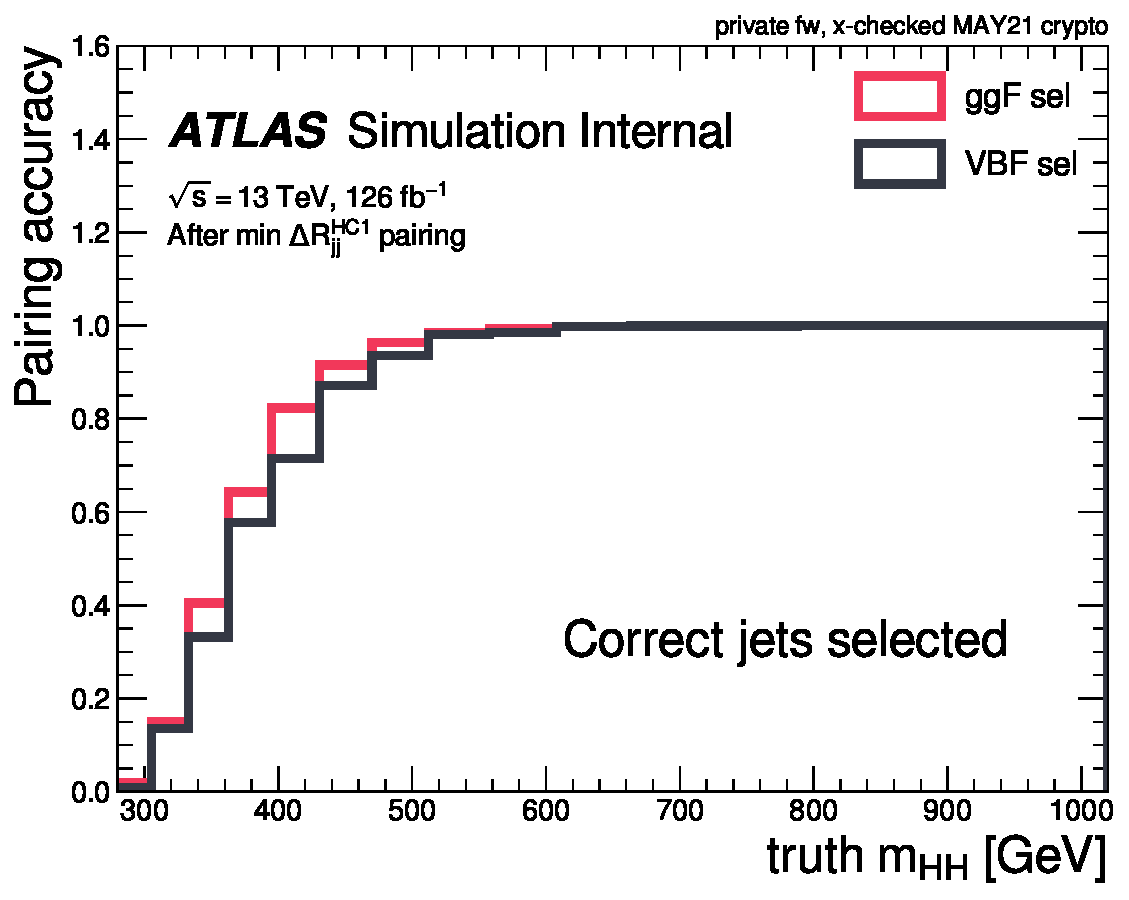
\includegraphics[width=0.5\textwidth]{figures/nr-int-note/selection/V2/acc_truth_mhh_exists_4b_only.pdf}
    \caption{Pairing accuracy as a function of truth \mhh, given that the correct jets have been selected. The ggF selection accuracy is derived from the ggF SM sample, and the VBF selection accuracy is derived from the VBF \kvv sample.}
    \label{fig:pairingAcc-mhh-exists-4b}
\end{figure}

\FloatBarrier

